\documentclass[pdf]{beamer}
\usepackage[utf8]{inputenc}
\usepackage{graphicx}
\usepackage[T1]{fontenc}      
\usepackage[francais]{babel}
\usepackage{graphicx}
\usepackage{circuitikz}
\usepackage[squaren, Gray]{SIunits}
\usepackage{sistyle}
\usepackage[autolanguage]{numprint}
\usepackage{pgfplots}
\usepackage{amsmath,amssymb,array}
\usepackage{wrapfig}

\usetheme{warsaw}
\mode<presentation>{}

\title{Projet 2 : concevoir un haut-parleur}
\subtitle{Pré-jury}
\author{Groupe 115.3}
\date{\today}

\begin{document}

\begin{frame}
	\titlepage
\end{frame}

\begin{frame}
	\frametitle{Etat d'avancement du projet}	

\end{frame}

\begin{frame}
	\frametitle{Recherche documentaire}
	\framesubtitle{La contre-réaction (ou contre réaction négative)}
	 
\end{frame}

\begin{frame}
	\frametitle{Recherche documentaire}
	\framesubtitle{La distorsion}
	% Contenu
\end{frame}
	
\begin{frame}
	\frametitle{Approximation de la fréquence de coupure}
	% Contenu
\end{frame}

\begin{frame}
	\frametitle{Modélisation du filtre passe-bas}

	\begin{minipage}{0.5\linewidth}
	{
		\center
		{
			\scalebox{0.50}{\begin{tikzpicture}[>=stealth]
			\begin{axis}[
					xmin=0,xmax=6,
					ymin=-8,ymax=8,
					axis x line=middle,
					axis y line=middle,
					axis line style=->,
					xlabel={$V$},
					ylabel={$t$},
					]
					
					\addplot[no marks,black,-] expression[domain=0:6,samples=1000]
							{((7.5)/(sqrt(1 + 1000^2 * 0.00001^2 * 400^2))) * (((-2.718^((-x)/(1000*0.00001)))/(sqrt(1 + 1000^2 * 0.00001^2 * 400^2))) 
							+ cos(atan(-1000*0.00001*400) + 400*x))} 
							node[pos=0.65,anchor=south west]{$$};
							
					\addplot[no marks,blue,-] expression[domain=0:6,samples=1000]
							{7.5 * cos(400 * x)} 
							node[pos=0.65,anchor=south west]{$$}; 

			\end{axis}
			\end{tikzpicture}}
		}
	}
	\end{minipage}
	
	\begin{flushright}
	\begin{minipage}{0.4\linewidth}
			-	$V_{out}$ est en retard de $\arctan{RC\omega}$ par rapport à $V_{in}$ ;
			- Le déphasage augmente avec la fréquence ;
	\end{minipage}
	\end{flushright}
	
	\hfill
	
	\begin{minipage}{0.5\linewidth}
	{
		\center
		{
			\scalebox{0.5}{\begin{tikzpicture}[>=stealth]
			\begin{axis}[
				xmin=0,xmax=1400,
				ymin=0,ymax=1.2,
				axis x line=middle,
				axis y line=middle,
				axis line style=->,
				xlabel={$f$},
				ylabel={$V_{out} / V_{in}$},
				]
				
				\addplot[no marks,green,-] expression[domain=0:1400,samples=100]
						{(1 + (2*3.14*x*100*0.00001)^2)^(-0.5)}
						node[pos=0.65,anchor=south west]{$$}; 
			\end{axis}
			\end{tikzpicture}}
		}
	}
	\end{minipage}
	
	\begin{minipage}{0.5\linewidth}
			- Atténue les hautes fréquences, laisse passer les basses fréquences ;		
	\end{minipage}

\end{frame}
	
\begin{frame}
	\frametitle{Modélisation du filtre passe-haut}
	
\end{frame}

\begin{frame}
	\frametitle{Dimensionnement du haut-parleur}
	% Contenu
\end{frame}

\begin{frame}
	\frametitle{Dimensionnement des bobines}
	

	\center{
\begin{minipage}{0.5\linewidth}
{\center{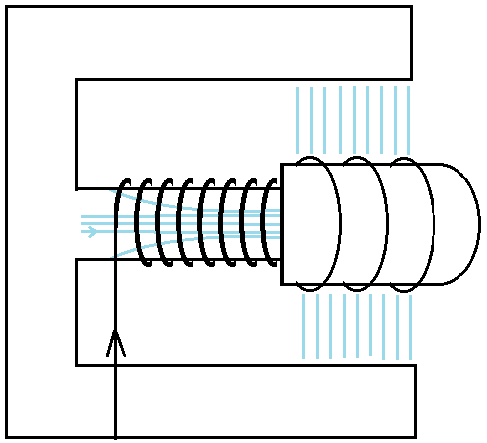
\includegraphics[scale=0.2]{hautparleur.png}}}
\end{minipage}\hfill
\begin{minipage}{0.5\linewidth}
\center{La bobine fixe joue un rôle d'électroaimant. Dans des conditions idéales, le champ total crée est $B = \unit{0.1143}{\tesla}$}
\end{minipage}
\\

 \vspace{4\baselineskip}
	
\paragraph{\textbf{Tableau récapitulatif}}
\small{\begin{center}
\begin{tabular}{c|c|c|c|c|c}
$$ & $N$ & $I$ & $R$ & $L$ & $L_{fil}$ \\
\hline
$Bobine fixe$ & $400$ & $\unit{2.5}{\ampere}$ & \unit{7.254}{\ohm} & $\unit{0.01475}{\henry}$ & $\unit{40.3}{\meter}$\\
\hline
$Bobine mobile$ & $ 118 $ & $\unit{0.1667}{\ampere}$ & $\unit{2.38}{\ohm}$ & $\unit{0.0734}{\henry}$ &\unit{12.6}{\meter}$\\
\end{tabular}

	\end{center}}
	}\\


\end{frame}

\end{document}
